\section{Durchführung}
\label{sec:Durchführung}

Der Versuch wird mit der Apparatur in Abbildung (3) durchgeführt.
Sie besteht aus einem Torsionsdraht, und einer daran aufgehangenen Kugel mit einem Permanentmagneten.

\begin{figure}[H]
 \centering
  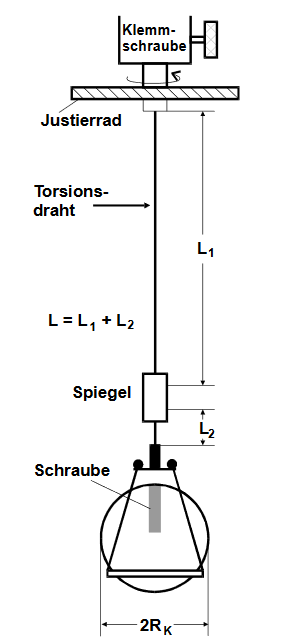
\includegraphics[height=8cm]{Screenshot (10).png}
  \caption{Messapparatur ohne Zeitmessvorrichtung.\cite{kent}}
  \label{fig:drill}
\end{figure}


\subsection{Bestimmung des Schubmoduls}
Zuerst wird sichergestellt, dass der Magnet vertikal in der Kugel liegt, damit das Erdmagnetfeld die Messung nicht beeinflussen kann.
Das System wird in Schwingung versetzt und mit einer elektronischen Stoppuhr wird die Periodendauer gemessen.
Eine Torstufe stellt sicher, dass die Zählung zum richigen Zeitpunkt beginnt.
Das dafür erforderliche Signal wird mit einer Lichtschranke erzeugt(s. Abbildung (4)).
Immer, wenn die Photoiode von einem Lichtstrahl getroffen wird, gibt sie ein Signal ab, welches mittels einer digitalen Schaltung auf die Torstufe geleitet wird.

\noindent Ist alles aufgebaut, wird der Spiegel mittels des Justierrades so eingestellt, dass der Lichtstrahl etwas neben die Photoiode fällt.
Lenkt man das System aus, indem man das Justierrad dreht, wird der Lichtstrahl an der Photoiode hinweg geführt zum Umkehrpunkt, und schließlich wieder zurück.
Somit ist nach dem dritten Impuls eine Periode vergangen, und die Zeit kann abgelesen werden.
Für diese Methode werden 10 Schwingungen gemessen. Es ist zu beachten, dass die Kugel nur um kleine Winkel ausgelenkt werden darf, und sie keine Pendelbewegungen ausführen darf.


\begin{figure}[H]
 \centering
  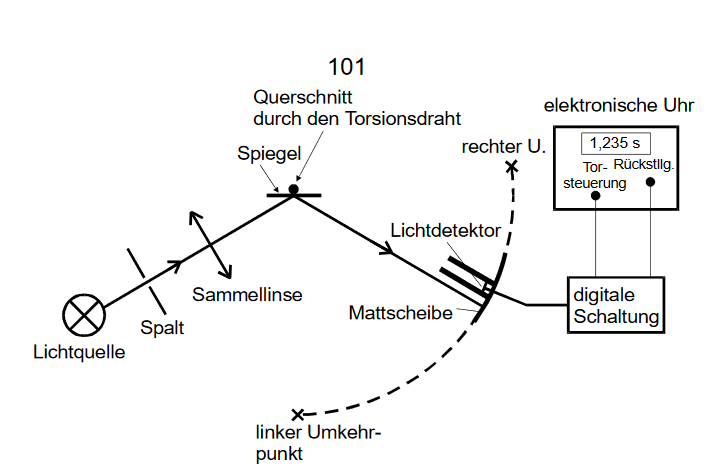
\includegraphics[height=8cm]{Screenshot (11).png}
  \caption{Prinzip der Messung der Periode.\cite{kent}}
  \label{fig:drill}
\end{figure}



\subsection{Bestimmung des magnetischen Momentes eines Permanentmagneten}
Das Magnetfeld wird von einer Helmholtz-Spule erzeugt (s. Abbildung (5)).
Diesmal muss der Magnet horizontal in der Kugel liegen, so dass die Dipolachse parallel zur Feldrichtung steht. Das System wird wie im Abschnitt vorher in Schwingung versetzt, nur diesmal werden für 5 verschiedene Stromstärken je 5 Perioden ermittelt.
Auch bei dieser Messung wird mit Kleinwinkelnäherung gerechnet, somit darf die Auslenkung nicht allzu groß sein.

\begin{figure}[H]
 \centering
  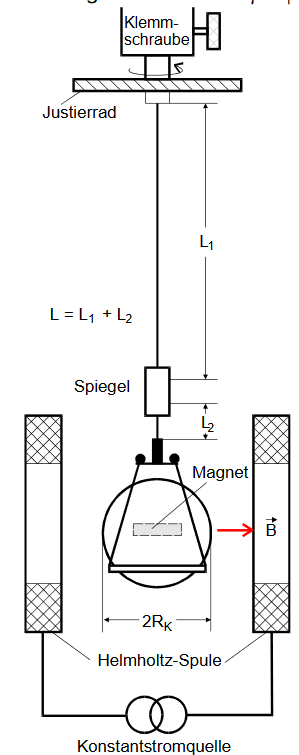
\includegraphics[height=8cm]{Screenshot (12).png}
  \caption{Messapparatur mit Helmholtz-Spule.\cite{kent}}
  \label{fig:drill}
\end{figure}